\chapter{Exciton-Polariton in simple lattice}\label{CHTWO}
%In this chapter, we find the nontrivial ground dispersion of exciton-polaritons by coupling the excitons and cavity photons in two separate periodic potentials. We then discuss the possible resulting phenomenona.
%In this chapter, we extend the Gross--Pitaevskii equation with complex valued potential and complex valued nonlinearity.
%The imaginary part of the potential describes the gain and loss of the exciton-polaritons, and the imaginary term of the nonlinear interaction defines the saturation of the gain from the reservoir.
In this chapter, we devote our focus on the exciton-polariton in the simple lattice which has one lattice site in per unit cell.
In the tight-binding model with the nearest neighbour hopping approach, this indicates one has one simple band in the spectrum.
In the following sections, instead of the discrete lattice approach, we consider the exciton-polariton in the continuous limit to include long-range interaction.

At the beginning of this chapter, we investigate the dispersion of exciton-polaritons in the case that the coupling between exciton part and cavity photon part is in two separate periodic potentials.
We find a nontrivial ground state in the middle of the Brillouin zone. We further investigate the corresponding dynamics of exciton-polaritons in this system.

In the rest part of this chapter, we extend the Gross--Pitaevskii equation with complex-valued potential and complex-valued nonlinearity.
The imaginary part of the potential describes the gain and loss of the exciton-polaritons, and the imaginary term of the nonlinear interaction defines the saturation of the gain from the reservoir.
We find that in such a configuration, the condensate phase may change if we tune the real or imaginary part of the nonlinearity.

\section{Multivalley engineering in semiconductor microcavities}\label{Ch2}
%
%---------------------------------------------------------------
%
%\subsection{Background}
As we know, photonic and electronic systems support many universal phenomena.
To mention a few, topological photonics has recently risen from ideas in the study of topological insulators~\cite{Lu:2014aa}, and the field of spintronics has been an inspiration for optical analogues for the optical spin Hall effect~\cite{Leyder:2007aa} and the development of photonic spin switches~\cite{Lagoudakis:2002aa,Amo:2010aa}.
While the advantages of spintronics for information processing remain promising, the flourishing field of valleytronics proposes to encode information in the valley degree of freedom of multivalley semiconductors~\cite{Behnia:2012aa,Nebel:2013aa}, including transition metal dichalcogenides (TMDs)~\cite{Xu:2014aa,Jones:2014aa,He:2014aa,Chernikov:2014aa}.
This raises the question of whether valleytronics is itself a universal concept that can also appear in suitably engineered photonic systems.

Recently, several works have attempted to hybridize light confined in planar microcavities with TMDs~\cite{Vasilevskiy:2015aa,Lundt:2016aa} resulting in exciton-polaritons with large binding energies.
Indeed, such a system is highly promising as a nonlinear photonic system operating at room temperature; however, the valleytronic features of multivalley semiconductors that occur at wave vectors given by the inverse crystal lattice constant are uncoupled from optical modes that are restricted to lower in-plane wave vectors inside the light cone.
Thus, one needs a different approach to engineer multiple valleys that are suitable for nonlinear optical valleytronics.
% The engineering of multiple valleys suitable for nonlinear optical valleytronics thus requires a different approach.

For this purpose, exciton-polaritons remain a good candidate as their relatively large micron-scale de Broglie wavelength gives them the advantage to be strongly manipulated by micron-scale potentials in microcavities.
Such potentials can be manipulated either by spatial modulation of the photon energy~\cite{Kaitouni:2006aa,Lai:2007aa} or the exciton energy~\cite{Balili:2007aa,Amo:2010aa,Assmann:2012aa,Cristofolini:2013aa,Askitopoulos:2013aa}.
Periodic potential arrays have been introduced~\cite{Lai:2007aa,Cerda-Mendez:2010aa} with various lattice geometries~\cite{Kim:2013aa,Cerda-Mendez:2013aa,Winkler:2016aa}, leading to several different phenomena, for example gap solitons~\cite{Ostrovskaya:2013aa,Tanese:2013aa}, flatbands~\cite{Jacqmin:2014aa}, and Bloch oscillations \cite{Flayac:2011aa,Flayac:2013aa}.
Researchers have also suggested several new devices \cite{Flayac:2013aa,Marsault:2015aa} and (theoretically) non-trivial topological properties~\cite{Karzig:2015aa,Nalitov:2015aa,Bardyn:2015aa,Bardyn:2016aa}.

In this chapter, we consider the behavior of exciton-polaritons in a microcavity where both the optical and excitonic components are separately manipulated by two periodic potentials.
These potentials can be achieved by ``proton implantation'' \cite{Schneider:2016aa}, in which the properties of QWs and semiconductor microcavities are spatially patterned after growth.
The different localization of photons and excitons by their respective potentials theoretically allows for a nontrivial overlap of their wave functions that depends on the in-plane momentum.
Remarkably, we can realize momentum-dependent coupling between excitons and cavity photons, which gives rise to the formation of nontrivial dispersion with degenerate ground states at non-zero momenta at the bottom of different valleys in the reciprocal space.

We further show that when considering TE-TM splitting, different valleys have different polarizations, analogous to the spin-valley coupling that forms the basis of valleytronics in 2D semiconductor systems.
For additional effects that arise from the unusual exciton-polariton dispersion in our system, we consider the behaviour of the system under incoherent excitation conditions.
Considering the inherent excitation case, it is known that exciton-polaritons may undergo BEC~\cite{Kasprzak:2006aa}, characterized by the breaking of U(1) phase symmetry and the appearance of a macroscopic coherent low-energy state.
Other symmetries may also be broken under BEC, both in exciton-polariton systems and other systems including spin symmetry breaking~\cite{Sadler:2006aa,Ohadi:2012aa}, translational symmetry breaking~\cite{Kanamoto:2003aa}, and angular momentum symmetry breaking~\cite{Butts:1999aa,Liu:2015aa}.
In our system, we find that there is also a spontaneous breaking of linear momentum symmetry, where the condensates can spontaneously choose between different valleys in the dispersion.
% We also show that under resonant excitation, the presence of a two-mode squeezing due to polariton--polariton interactions leads to the onset of non-classical quantum correlations.

%
%-----------------------------------------------------------------------------------------
%
\subsection{Dispersion of lattice exciton-polaritons}
Let us begin by considering a 1D system of cavity photons and QW excitons~\cite{Tanese:2013aa}, which have potentials with the same periodicity but different alignment in energy, as shown in Fig.~\ref{fig:CH2_Fig1}(a).
Using the Bloch theory and the model of coupled harmonic oscillators, we can apply the central equation in~\cite{kittel:1966aa} and solve the eigenvalue problem of the system.
In a brief form this equation reads:
%
\begin{eqnarray}
	\begin{pmatrix}
		\lambda_{C}-\mi\hbar/\tau_C-E & \Omega \\
		\Omega & \lambda_{X}-\mi\hbar/ \tau_X -E
	\end{pmatrix}
	C_k
	 + \sum_{G}
	\begin{pmatrix}
		\tilde{V}_{C}\left( G \right) & 0 \\
		0 & \tilde{V}_X\left( G \right)
	\end{pmatrix}
	C_{k-G}=0,
	\label{eq:CH2_SP1}
\end{eqnarray}
%
where $\lambda_{C}=\frac{\hbar^{2}k^{2}}{2m_{C}}$ and $\lambda_{X}=\frac{\hbar^{2}k^{2}}{2m_{X}}$ are the kinetic energy terms of the photonic and excitonic counterparts, respectively.
Parameters $\tau_{C,X}$ are the lifetimes of the cavity photons and excitons, $\Omega$ is the exciton-photon (Rabi) coupling constant, and $\tilde{V}_C\left( G \right)$ and $\tilde{V}_{X}\left( G \right)$ are the Fourier components of the potentials for the cavity photons and excitons in real space.
The summation is over $G$ , which is the reciprocal lattice vector of different order.
The reciprocal lattice vector is the same because we apply the same periodicity for the exciton and photon potential. The vector $C_{k}$ denotes the exciton and photon components in the polariton mode with different $k$, and $E$ is the eigenenergy of the exciton-polariton mode.

%
%
%
\begin{figure}[ht]
\centering
	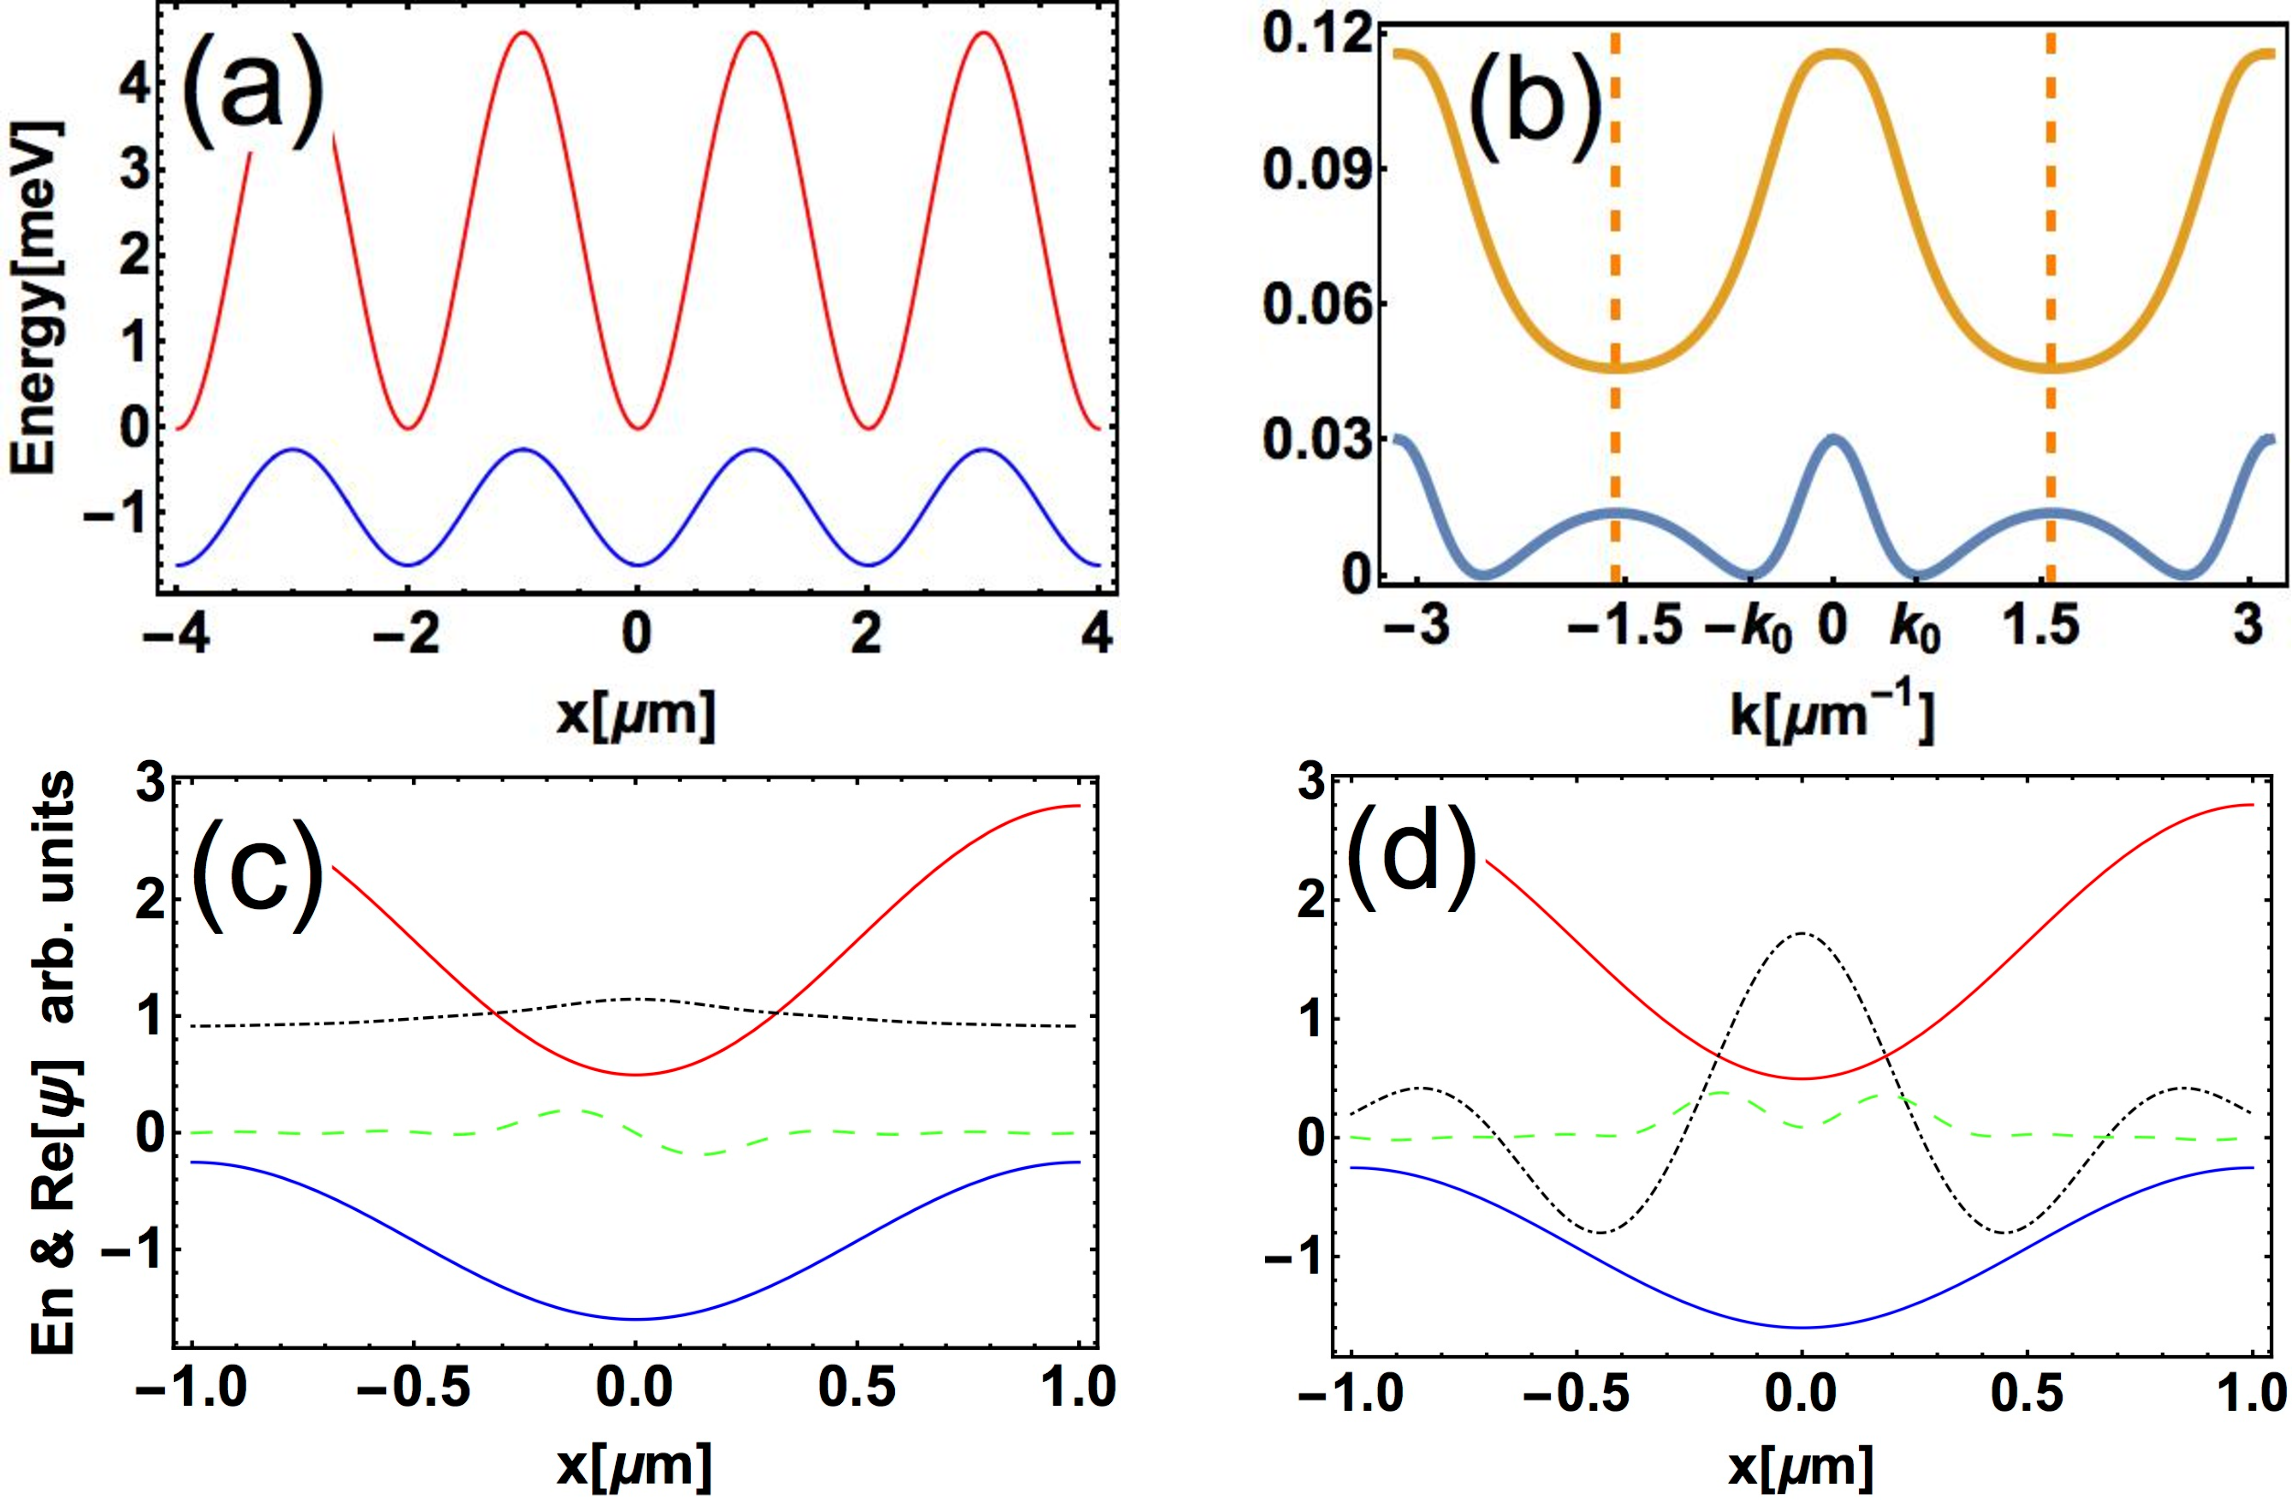
\includegraphics[width=0.79\linewidth]{Fig/Ch2/fig1.pdf}
	\caption[Potential setting, eigenenergy, and eigenstate of the system]{(a) Potential profiles for QW excitons (red) and cavity photons (blue). (b) Dispersion of the lowest-energy exciton-polaritons (blue), and the imaginary part of the polariton energy as a function of $k$ (yellow). The dashed vertical lines label the edges of the first Brillouin zone. (c, d) Real part of the wave function of the cavity photons (black dot-dashed line) and excitons (green dashed line) in a single lattice period with (c) $k=0$ and (d) $k$ at the edge of the Brillouin zone. Red and blue curves are the potentials of the excitons and cavity photons. The figure is taken from~\cite{Sun:2017ab}.}
	\label{fig:CH2_Fig1}
\end{figure}
%
%
%

After solving the eigenvalue problem with a truncation of a finite number of $G$ (see details in Appendix~\ref{AP:A1}), we find the dispersion of the system of exciton-polaritons in $k$-space, as shown in Fig.~\ref{fig:CH2_Fig1}(b), and the wave functions of the photons and excitons, as shown in Fig.~\ref{fig:CH2_Fig1}(c, d).
One should note that the excitonic dispersion is nearly flat on the $\mu m^{-1}$ scale, such that excitons are well localized on the minima of their potential.

In the meantime, cavity photons can also be localized depending on their momentum, which makes the coupling of photons and excitons momentum-dependent.
As Fig.~\ref{fig:CH2_Fig1}(b) shows, the dispersion is characterized by two minima at non-zero wave vectors, $k=k_0$.
In the following sections, we will show that this peculiar dispersion leads to non-trivial effects such as spontaneous momentum symmetry breaking upon exciton-polariton condensation.
%This result is one of the important result in this manuscript and in the following we show that this peculiarity

%
%---------------------------------------------------------------------------------
%
\subsection{Polariton BEC in the thermal equilibrium limit}
Before considering the structure of the dispersion in 2D lattices, it is helpful for us to understand the consequences of the dispersion shown in Fig.~\ref{fig:CH2_Fig1}(b) for the 1D scenario.
Here, we begin by considering the behavior of the system under non-resonant pumping, with which polariton condensation can be expected in the lattice~\cite{Lai:2007aa}.
Because of their finite lifetime, exciton-polaritons are non-equilibrium systems and so would not necessarily form in the ground state~\cite{Maragkou:2010aa}; however, at high densities, energy relaxation is typically enhanced to the ground state~\cite{Winkler:2016aa}.
In this section, we give a qualitative argument in the limit of thermal equilibrium~\cite{Sun:2017aa}.
%This is only intended to be used as qualitative insight for more accurate non-equilibrium modeling, which we will present in the latter sections.

From Eq.~\eqref{eq:CH2_SP1} we get the dispersion relationship, $E_k$, in the linear regime [shown in Fig.~\ref{fig:CH2_Fig1}(b)]. Then the Hamiltonian of the system can be written as
%
\begin{equation}
	\label{eq:CH2_H-2}
	%\hspace{-3mm}
	\hat{\mathcal{H}}=\sum_k  E_k \hat{a}_k^\dag \hat{a}_k +\alpha \hat{a}_k^\dag \hat{a}_k^\dag \hat{a}_k \hat{a}_k + 2\alpha \sum_{k' \neq k} \hat{a}_k^\dag \hat{a}_{k'}^\dag \hat{a}_k \hat{a}_{k'},
\end{equation}
%
where we introduce polariton--polariton interaction with the strength $\alpha$. The factor $2$ in Eq.~\eqref{eq:CH2_H-2} is characteristic of the momentum space scattering processes~\cite{Whittaker:2005kg} and can be considered as a permutation of $\hat{a}_k^\dag \hat{a}_{k'}^\dag \hat{a}_k \hat{a}_{k'}$.
%
%
%
\begin{figure}[ht]
	\centering
	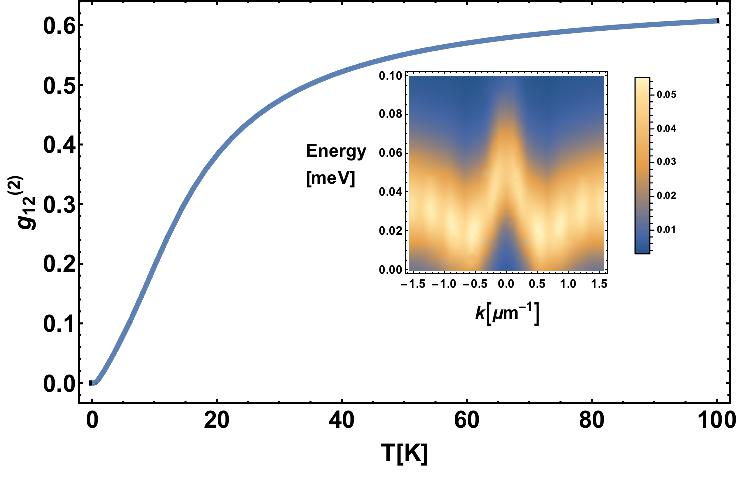
\includegraphics[width=0.65\linewidth]{Fig/Ch2/Fig2.jpg}
	\caption[Temperature-dependent $g_2$ function]{Second-order correlation function as a function of temperature. The total number of exciton-polaritons is fixed at $n=100$. The inset plots the low-density result with the total number of polaritons restricted to $n=3$, compared with the dispersion in Fig.~\ref{fig:CH2_Fig1}(b). The figure is taken from~\cite{Sun:2017ab}.}
	\label{fig:CH2_TMFig}
\end{figure}
%
%
%

At zero temperature, one can expect that only the two lowest energy momentum states at $k_1= -k_0$ and $k_2=k_0$ are populated, where $k_0$ is the right minimum valley of the blue curve in Fig.~\ref{fig:CH2_Fig1}(b). 
Then the energy of the system can be written as
%
\begin{align}
	E\left( n_1 , n_2 \right) &= nE_{k_1} + \alpha \left( n_1^2 +n_2^2 - n + 4n_1 n_2 \right),
	\label{eq:CH2_E-2}
\end{align}
%
where we define $n_{k_1} = n_1 $, $n_{k_2} = n_2$, and the total population $n =n_1 +n_2$.
It is easy to see that when $\rho=\left( n_1-n_2 \right)/n = \pm 1$, the system achieves its minimum energy. 
%The lowest energy state thus appears when $\rho=\left( n_1-n_2 \right)/n$ achieves its extreme value of $\pm 1$. 
In other words, at zero temperature, one can expect that the system would spontaneously choose the state with all the polaritons at either $k_1$ or $k_2$. 
This result can be further confirmed by calculating the second-order correlation function and spectrum corresponding to the Hamiltonian in Eq.~\eqref{eq:CH2_H-2}, as shown in Fig.~\ref{fig:CH2_TMFig} (see Appendix~\ref{AP:A2} for details of the calculation).

% 
%--------------------------------------------------------------------------------------
% 

\subsection{Non-equilibrium model of polariton BEC}

%Exciton-polaritons have a finite lifetime and consequently form non-equilibrium condensates.
In models with weak energy relaxation, it is not necessary to reach the actual ground state of the system~\cite{Krizhanovskii:2009aa,Maragkou:2010aa} due to the finite lifetime of exciton-polaritons.
In this section, we further investigate the behaviour of the system using a stochastic quantum treatment and accounting for various scattering processes (see Appendix~\ref{AP:A4}).
We consider an $\rm{InGaAlAs}$ alloy-based microcavity and use the following parameters during calculation: sound velocity $c_s=5370$ m/s~\cite{Hartwell:2010aa}, and $\gamma=i\hbar/\tau=\hbar/18$ ps$^{-1}$~\cite{Gao:2012aa}.

%
%
%
\begin{figure}[ht]
\centering
	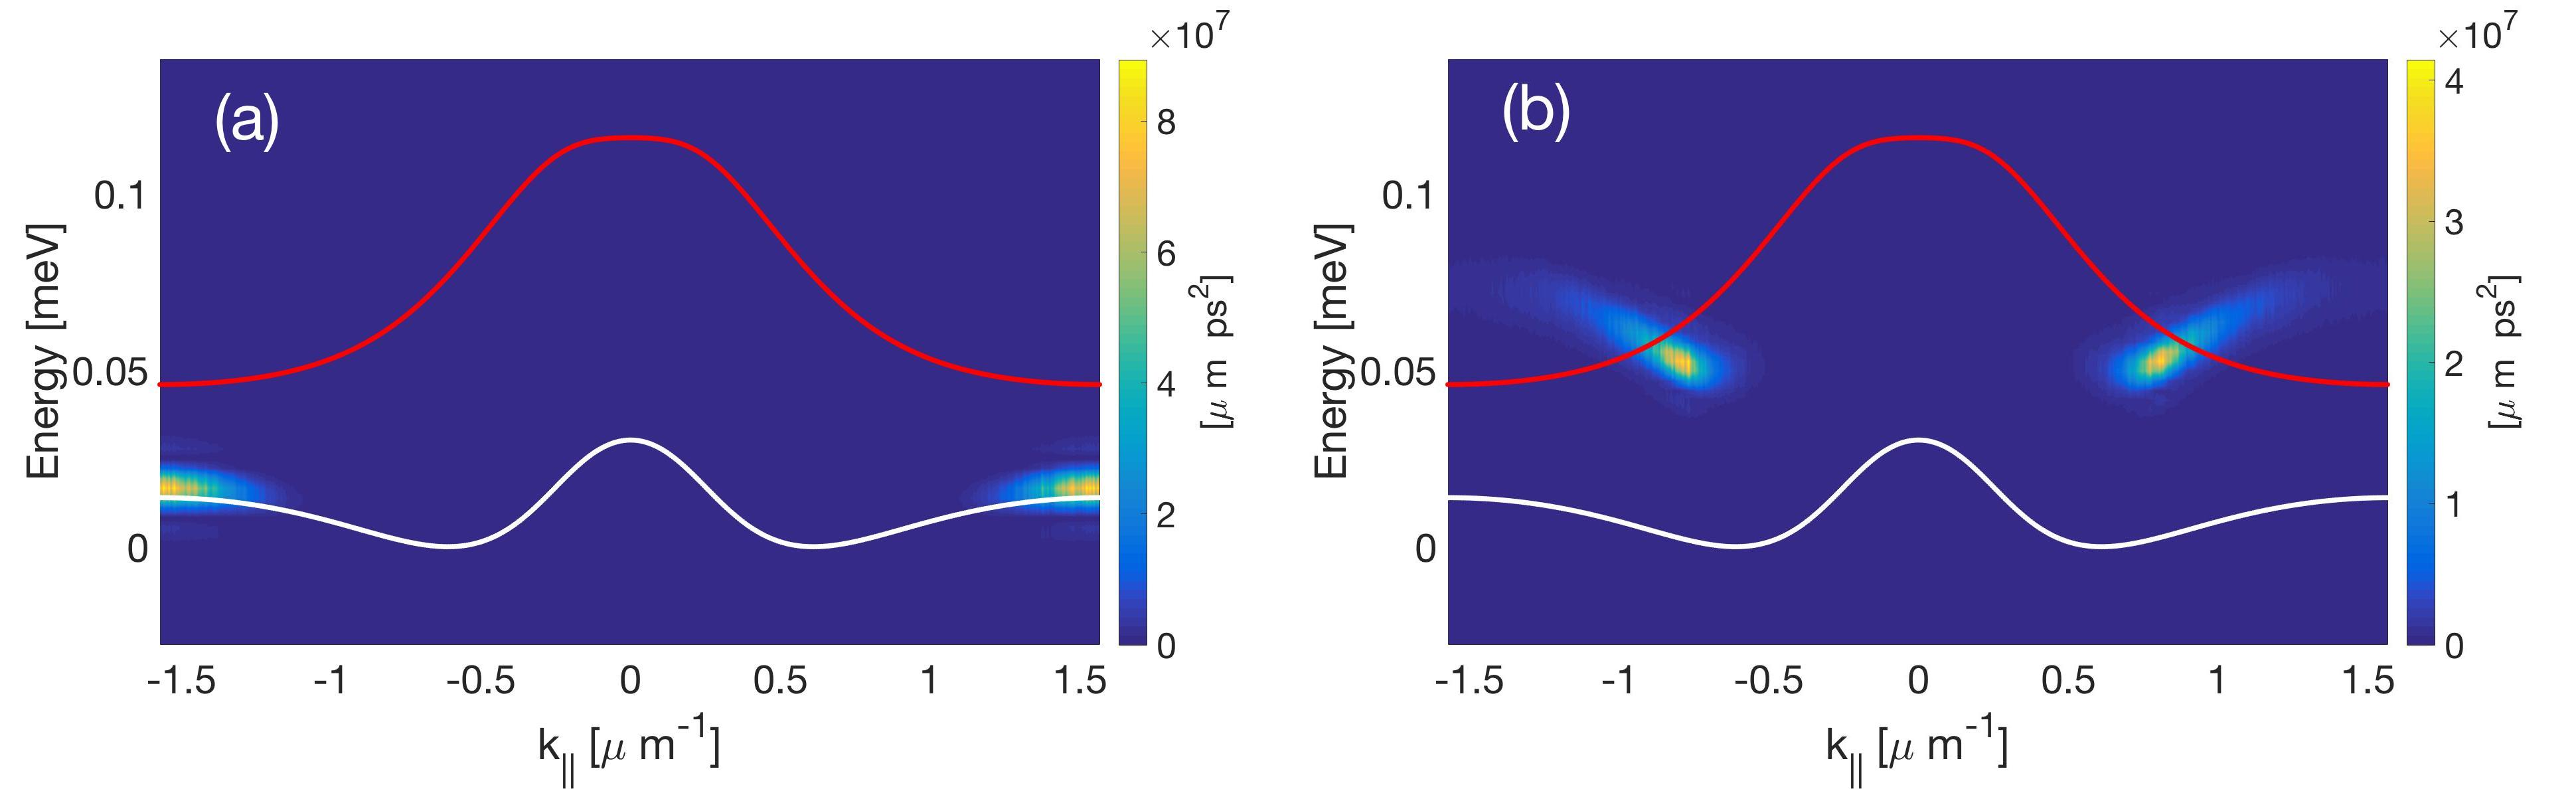
\includegraphics[width=0.99\linewidth]{Fig/Ch2/Fig3.jpg}
	\caption[Exciton-polariton spectra]{Distribution of exciton-polaritons localized in the potential profile shown in Fig.~\ref{fig:CH2_Fig1}(b) in the regime of homogeneous incoherent excitation of the system at steady state (1500 ps) including acoustic phonon-assisted scattering.
	Polariton--polariton interaction is switched (a) off and (b) on by setting $\alpha$ to zero and non-zero, respectively.
Red curves indicate the $k$-dependence of the decay rates, and white curves show the exciton-polariton dispersion in the linear regime.
	Exciton-polariton condensates form in the reciprocal space at $k_\parallel\approx \pm 0.74$ $\mu$m$^{-1}$. The figure is taken from~\cite{Sun:2017ab}.}
\label{fig:CH2_Fig4}
\end{figure}
%
%
%

In Fig.~\ref{fig:CH2_Fig4}(a), we turn off the polariton--polariton interaction and see that, in this case, there is no blueshift and the particles occupy mostly the edge of the Brillouin zone. 
This happens because particle lifetime increases with an increase of $|k_{\parallel}|$ with a corresponding decrease of the decay rate, see red curves in Fig.~\ref{fig:CH2_Fig4}.
However, if we account for interaction, we achieve degenerate condensation at $k=\pm k_0$ points due to the interplay of particle lifetime and interactions, as shown in Fig.~\ref{fig:CH2_Fig4}(b). 
Exciton-polaritons also blueshift in energy [compared with Fig.~\ref{fig:CH2_Fig4}(a)] due to this interaction.

One interesting point is that if we change the potential profiles for the excitons and photons, we can achieve different points of condensation; in particular, we can make particles condense at $k=0$ and $k=k_{BZ}$ (see Appendix~\ref{AP:A5}).

Although the condensation of polaritons to non-zero momentum states has been observed previously~\cite{Liu:2015aa,Maragkou:2010aa,Kusudo:2013aa}, in those observations it was a purely non-equilibrium effect.
In our work, on the other hand, condensation to non-zero momentum takes place even in the limit of thermal equilibrium, that is, with strong energy relaxation. 
Furthermore, since the non-zero momentum states are the true ground state of the system, they are likely to be highly stable after they have formed, particularly in polariton systems close to thermal equilibrium. 
This may include the previously developed long-lifetime inorganic microcavities~\cite{Nelsen:2013aa} as well as organic systems~\cite{Kena-Cohen:2010aa} with faster energy relaxation processes~\cite{Lanty:2008aa}.

%
%----------------------------------------------------------------------------------------- 
%
% \section{Entanglement generation: Resonant excitation}
% The two degenerate dispersion minima in the first Brillouin zone (as shown in Fig.~\ref{fig:CH2_Fig1}(b) and also in Fig.~\ref{fig:CH2_TMFig}) allow for the study of controlled entanglement in the system.
% Indeed, we can assume that each minimum is driven by a coherent laser with large enough spatial extension, and thus we can consider only two quantum modes as described by the creation operators $\hat a_{1}^{\dag}$ and $\hat a_{2}^{\dag}$.
% %
% %
% %
% \begin{figure}[ht]
% \centering
% 	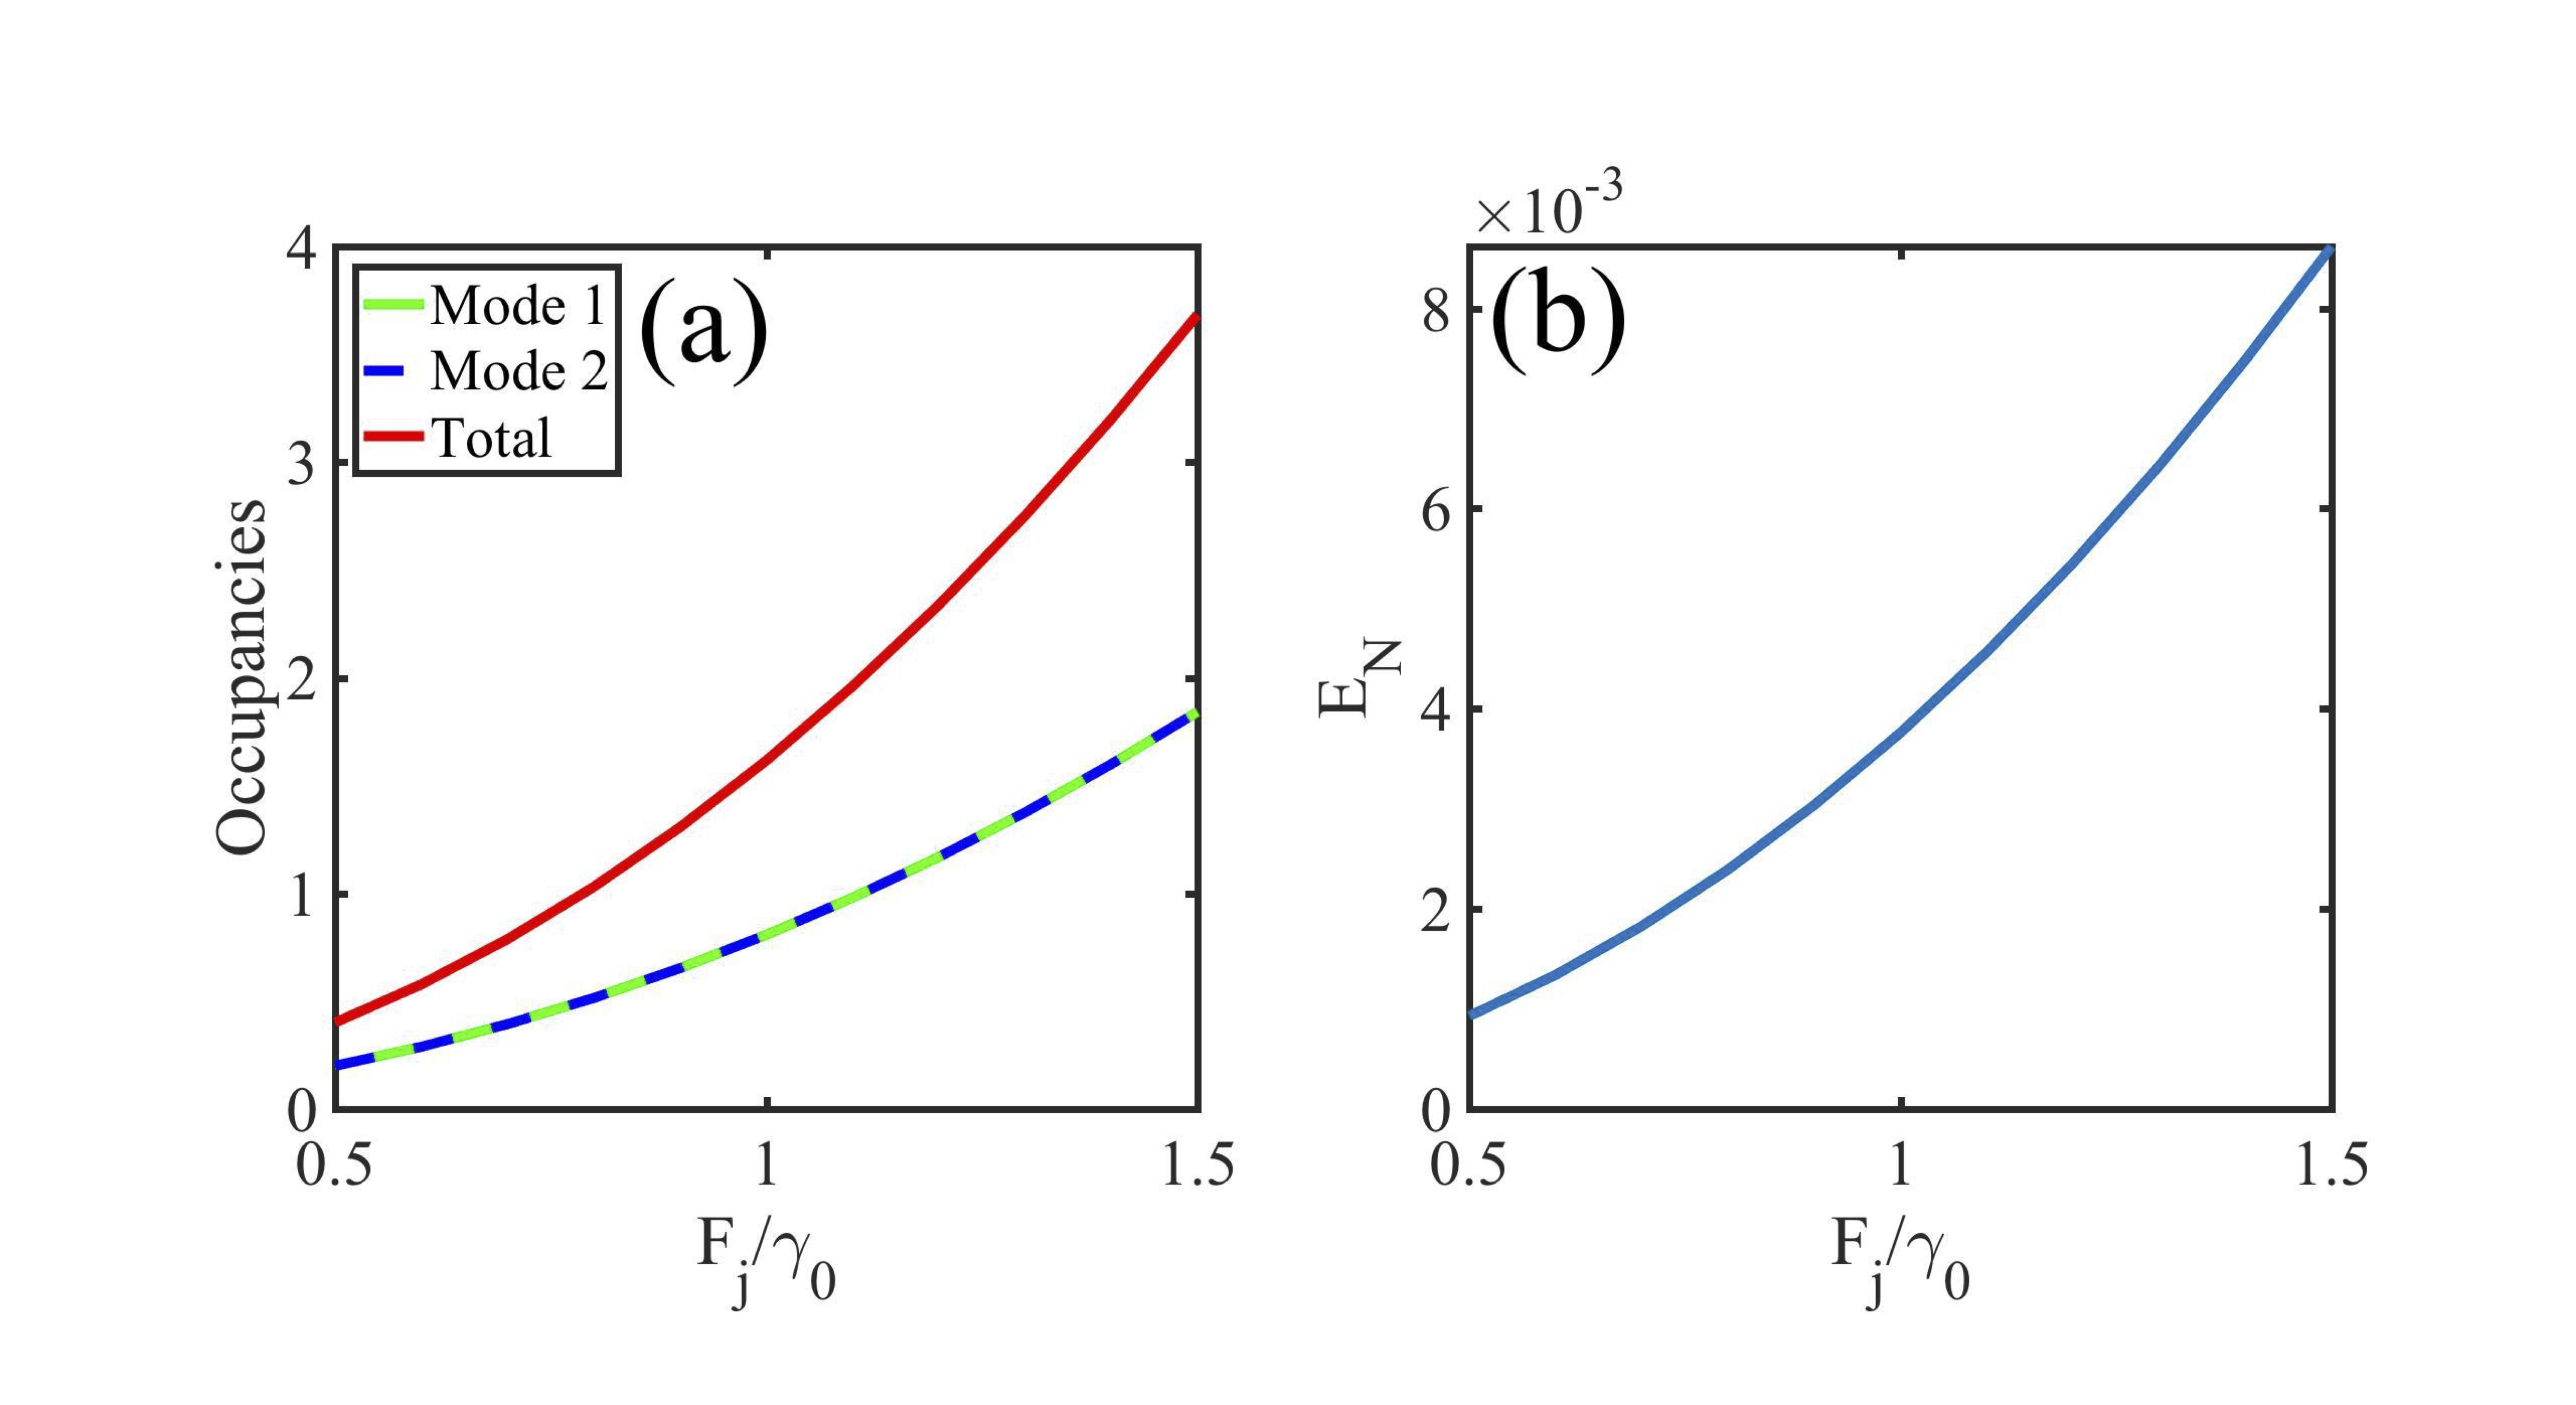
\includegraphics[width=0.89\linewidth]{Fig/Ch2/Fig4.jpg}
% 	\caption[Entanglement result]{Entanglement generation between the particles localized in the dispersion minima under resonant excitation (see Fig.~1a,c, and d). (a) Average mode occupancies found from the numerical solution of Eq.~\eqref{eq:CH2_rhot} in steady state, and (b) logarithmic negativity versus increasing driving strength. The parameters are $\gamma_0=8.6$ ps$^{-1}$, $\Delta_1=\Delta_2=\hbar\gamma_0$, and $\alpha=4.5\times10^{-4} {\rm{meV}} $.  }
% 	\label{fig:CH2_Entanglement}
% \end{figure}
% %
% %
% %
% In order to describe the dynamics of the system, we use a dissipative master equation in the form
% %
% \begin{equation}
% 	\label{eq:CH2_rhot}
% 	i\hbar\frac{{\partial \hat \rho }}{{\partial t}} = [ {\hat {\cal H}',\hat \rho } ] - \frac{{i{\hbar\gamma _0}}}{2}\sum\limits_{j = 1,2} {\hat {\cal D}\left[ {{{\hat a}_j}} \right]\hat \rho },
% \end{equation}
% %
% where the deterministic evolution is described by the Hamiltonian
% %
% \begin{eqnarray}
% 	 {\cal \hat H}' &=& \sum\limits_{j = 1,2} {-{\Delta _j}\hat a_j^\dag {{\hat a}_j} + \alpha\hat a_j^\dag \hat a_j^\dag {{\hat a}_j}{{\hat a}_j}}  + {F_j}\left( {\hat a_j^\dag  + {{\hat a}_j}} \right) +4\alpha\hat a_1^\dag \hat a_2^\dag {{\hat a}_2}{{\hat a}_1},
% 		\label{eq:CH2_Hres}
% \end{eqnarray}
% %
% which is similar to Eq.~\eqref{eq:CH2_H-2} after including the pumping terms, and in the frame rotating with laser frequency, assuming $F_j\in\mathbb{R}$ and with $\Delta_j$ defined as the laser/modes detuning.
% We further assume $\Delta_1=\Delta_2=0$ and $F_1=F_2$ for simplicity.
% %
% It is crucial that the Hamiltonian in Eq.~\eqref{eq:CH2_Hres} includes two kinds of interaction terms. 
% The first one ($\alpha$) stands for the interaction between exciton-polaritons located within the same minimum valley, while the second term ($4\alpha$) accounts for the cross-interactions between the minima, which fulfills energy momentum conservation, by the exchange of the wave vector $+k\rightarrow-k$ and no energy change (see Appendix~\ref{AP:A3}). 
% Physically, the latter term corresponds to the cross-Kerr interaction, which is known to induce two-mode squeezing~\cite{Wang:2015aa}, and therefore continuous variable entanglement is expected to occur in the reciprocal space. 

% The indeterministic part of the evolution is described by the last term in Eq.~\eqref{eq:CH2_rhot}, $\hat{\cal{D}}\left[ {{{\hat a_j}}} \right]\hat \rho = \{\hat a_j^\dag {{\hat a_j}},\hat \rho\} - 2{{\hat a_j}}\hat \rho \hat a_j^\dag$ corresponding to the Lindblad super operators that account for polariton decay due to interaction with their environment. 
% The continuous variable entanglement is quantified via logarithmic negativity~\cite{Vidal:2002aa}, $E_{\cal N}=\log_2{|| {\hat \rho^{{\Gamma _{2}}}} ||_1}$, where ${\hat \rho^{{\Gamma _{2}}}}$ is the partial transpose of $\hat \rho$ with respect to the second mode and ${|| {\hat \rho^{{\Gamma _{2}}}} ||_1}$ is its trace norm. 
% In Fig.~\ref{fig:CH2_Entanglement}, we present steady-state numerical solutions with regard to Eq.~\eqref{eq:CH2_rhot} showing the average mode occupations in panel (a) and the corresponding values of $E_{\cal N}$ in panel (b) for increasing pump amplitudes.
% Direct proof of entanglement is from the observation of a monotonous increase in both of the quantities. 
% Importantly, no state other than the one targeted by the laser can be reached by potential parametric processes which would violate the energy conservation.

% 
%----------------------------------------------------------------------------------------- 
% 
\subsection{Polariton polarization and dispersion in a 2D lattice}
In this section, we extend the dispersion calculation into a 2D square lattice structure.
Figure~\ref{fig:CH2_Fig2D}(a) shows the energy of the system ground state in the first Brillouin zone (see also Appendix~\ref{AP:A5}).
Here we can identify four energy minima at the bottom of different valleys in the reciprocal space.
%
%
%
\begin{figure}[ht]
	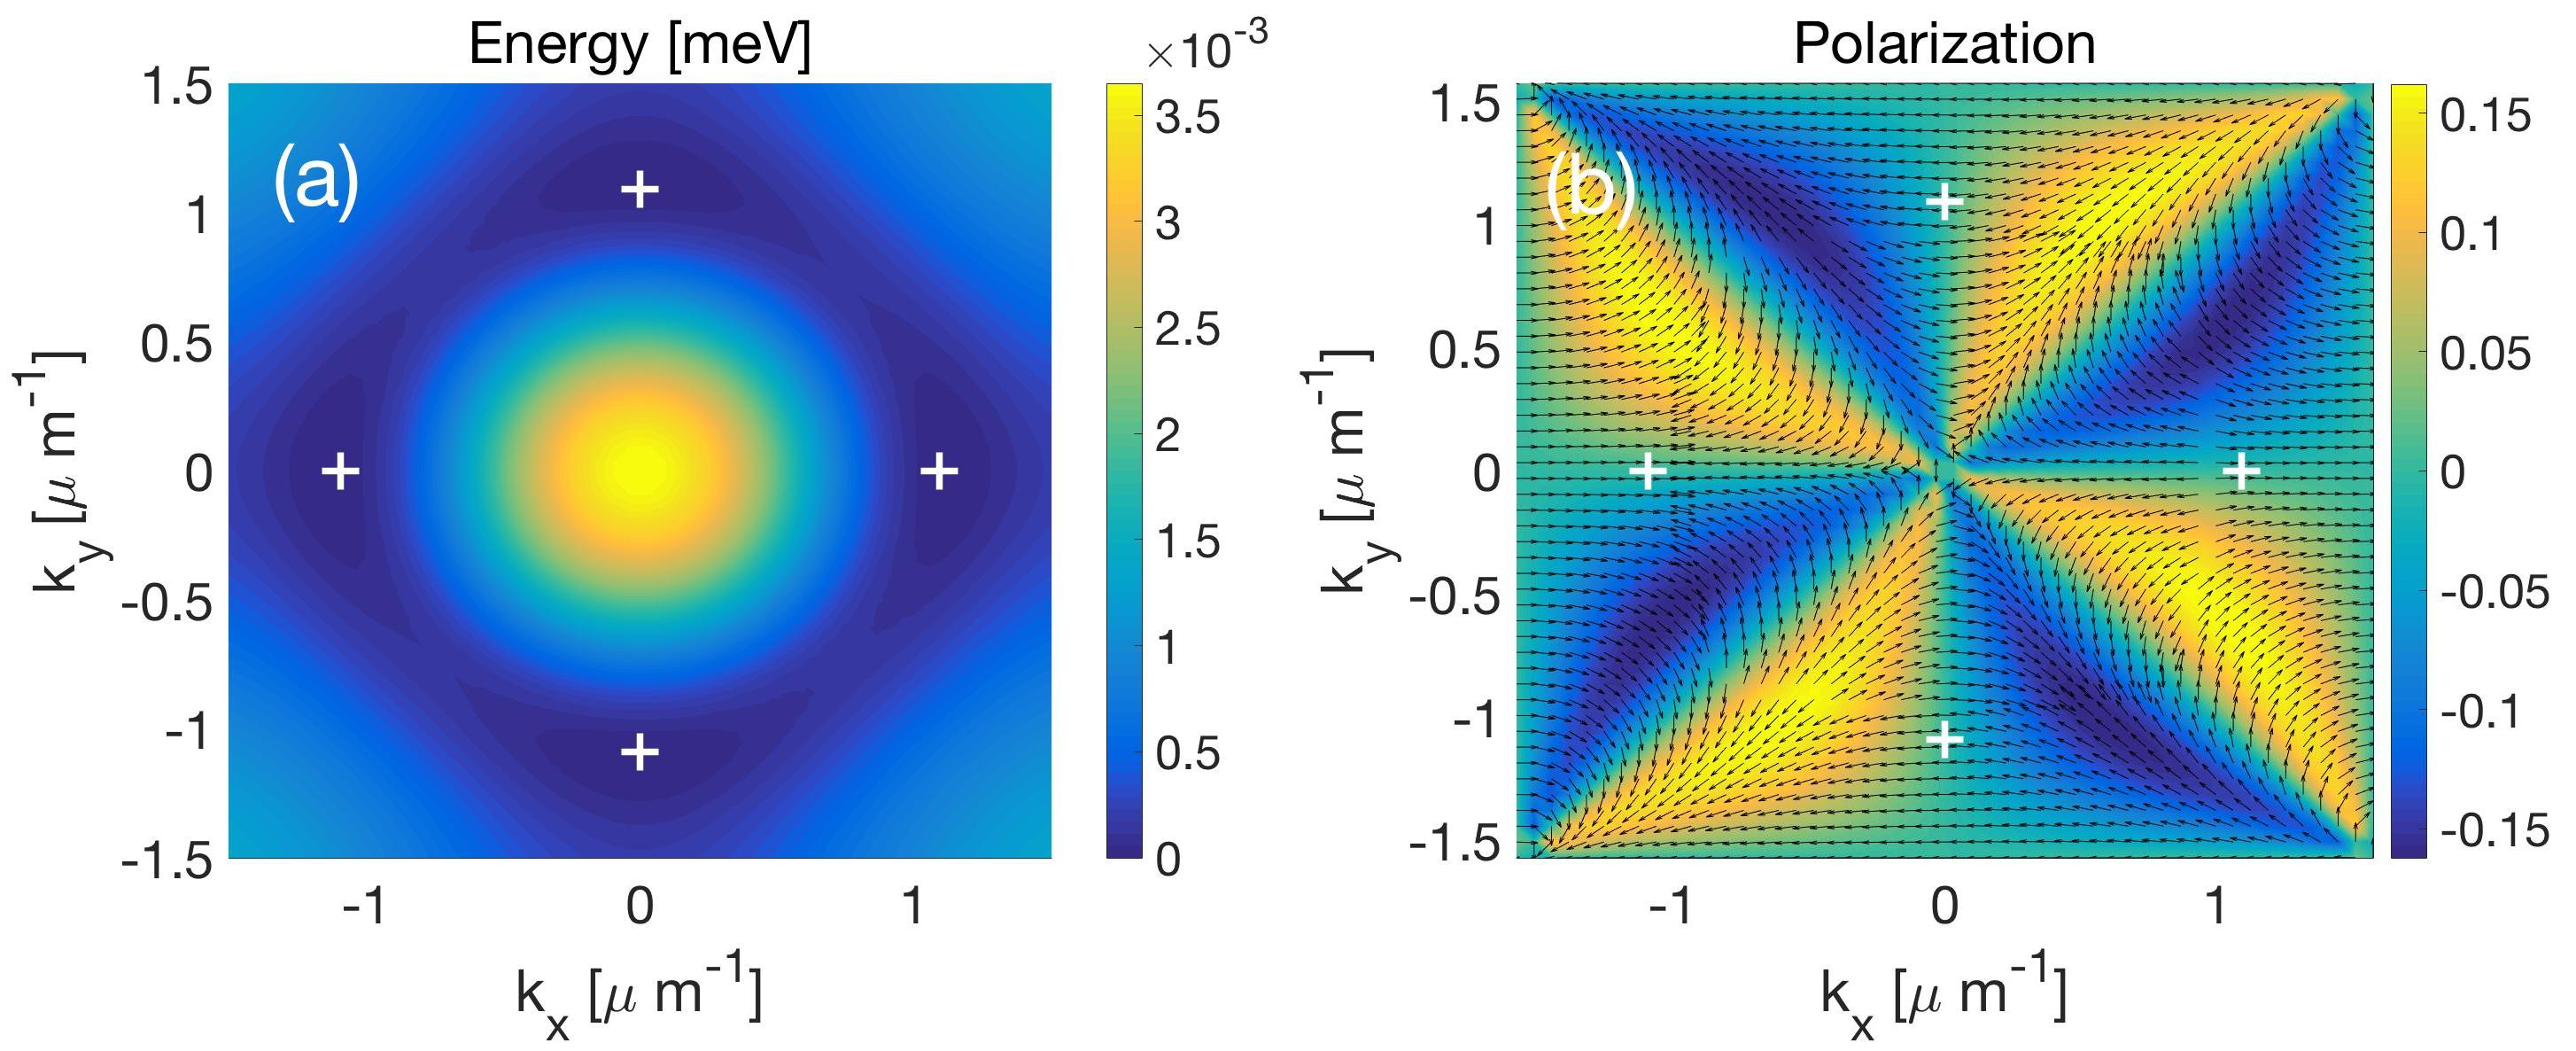
\includegraphics[width=0.99\linewidth]{Fig/Ch2/Fig5.jpg}
\caption[Illustration of multivalley coupling]{Illustration of multivalley coupling. (a) Energy dispersion in 2D in the first Brillouin zone, and (b) corresponding polarization chart. The arrows in (b) show the polarization in $x$- and $y$-directions, and colors represent the polarization in the $z$-direction. The white crosses mark the minima of the energy dispersion. The figure is taken from~\cite{Sun:2017ab}.}
\label{fig:CH2_Fig2D}
\end{figure}
%
%
%
A fundamental feature of 2D semiconductors for valleytronics is the spin-valley coupling that allows different valleys to be excited with light in different polarizations.
%In exciton-polariton systems, it is well-known that TE-TM-polarized modes are split in energy.
%This splitting can be described by a spin-orbit coupling Hamiltonian acting on the photon spin degree of freedom, which can be written as
We introduce the TE-TM splitting in our model to investigate its consequences. The corresponding Hamiltonian is
%
\begin{equation}
\label{eq:CH2_TE_TM}
\mathcal{H}_{TE-TM}=\left(\begin{array}{cc}0&\Delta\left(\frac{\partial}{\partial x}-\mi\frac{\partial}{\partial y}\right)^2\\\Delta\left(\frac{\partial}{\partial x}+\mi\frac{\partial}{\partial y}\right)^2&0\end{array}\right).
\end{equation}
%

After accounting for this splitting, we obtain the polarization structure of the lowest energy band, as shown in Fig.~\ref{fig:CH2_Fig2D}(b).
Here we note that the different valleys have different polarizations, which implies that they can be selectively excited by a resonant excitation with specific polarization.
The geometry of the lowest energy pseudospin should allow to form such patterns as skyrmions~\cite{Flayac:2013aa,Cilibrizzi:2016aa} or spin whirls~\cite{Cilibrizzi:2015aa} under pulsed-resonant excitation.

%
% ---------------------------------------------------------
%
\subsection{Summary}
In this chapter, we have considered the formation of exciton-polaritons in a semiconductor microcavity with separate spatially patterned potentials for cavity photons and excitons.
This separated confinement of cavity photons and excitons allows us a momentum-dependent coupling that gives rise to a unique shape of the dispersion, in which degenerate ground states appear at non-zero momenta.
We studied two different limits corresponding to strong and weak energy relaxation.
In the limit of strong energy relaxation, a simple equilibrium theoretical model predicts spontaneous symmetry-breaking in momentum space.
In the limit of weak energy relaxation, a non-equilibrium model accounting for phonon scattering processes shows that the system gives non-equilibrium condensation at a non-zero wave vector.
% Treating exciton-polaritons as an open quantum system, we also showed that correlations between the modes in reciprocal space can occur.
At last, considering exciton-polaritons in a 2D square lattice, we predicted the formation of a multivalley-dispersion.
Here, different valleys exhibit different polarizations, which, in principle, allows us to selectively excite the system with a polarized laser, and forms a foundation for exciton-polariton valleytronics.


